\subsection{Attention backward pass}
\label{sec:bwd}



\subsubsection{Feeds and Speeds}

Similar to the forward pass, we first provide intuition for our kernel design and optimizations by analyzing the roofline, based on the throughput of the matmul units (tensor cores), shared memory (smem), and exponential unit.

Let the tile shape along the sequence length dimension of $\vQ$ and $\vK$ be $M \times N$, and let the head dimension be $d$. We analyze the compute and memory traffic requirements to identify the performance bottleneck. Unlike for the forward pass, we make the assumption that $M = N = d = 128$ to simplify the formulas for the smem cycle count, although we retain variable names for clarity.

\noindent\textbf{MMA compute.}
The backward pass performs five matrix multiply-accumulate (MMA) operations per iteration. Each MMA involves an $M \times N$ matrix, an $M \times d$ matrix, and an $d \times N$  matrix (varying which one is the output matrix), requiring $2MNd$ floating-point operations. With a tensor core throughput of 8192 FLOPs per cycle, the total compute time is
{\setlength{\abovedisplayskip}{2pt}%
 \setlength{\belowdisplayskip}{2pt}%
 \setlength{\abovedisplayshortskip}{2pt}%
 \setlength{\belowdisplayshortskip}{2pt}%
\begin{equation}
    T_{\text{MMA}} = \frac{10MNd}{8192} \text{ cycles}.
\end{equation}}

\noindent\textbf{Shared memory traffic.}
Of the five MMAs, three of them -- $\vS^\top = \vK \vQ^\top$, $\vdP^\top = \vV \vdO^\top$, and $\vdQ = \vdS \vK$ -- are shared-shared (SS) operations where both operands are read from shared memory, while two -- $\vdV = \vP^\top \vdO$ and $\vdK = \vdS^\top \vQ$ -- are tensor-shared (TS) operations where operand $A$ is read from tensor memory and operand $B$ from shared memory. The SS MMAs read in total $2Md + 3Nd + MN$ elements from shared memory, while the TS MMAs read in total $2Md$ elements from shared memory. At a shared memory bandwidth of 128 bytes per cycle and with each element being 2 bytes (bf16), this contributes
{\setlength{\abovedisplayskip}{4pt}%
 \setlength{\belowdisplayskip}{4pt}%
 \setlength{\abovedisplayshortskip}{3pt}%
 \setlength{\belowdisplayshortskip}{3pt}%
\begin{equation}
    T_{\text{smem,MMA}} = \frac{4 M d + 3 N d + M N}{64} \text{ cycles}.
\end{equation}}
Additionally, the algorithm writes the intermediate gradient $\vdS$ of size $M \times N$ to shared memory in bf16, requiring $2MN$ bytes or $MN/64$ cycles. The gradient $\vdQ$ of size $M \times d$ is written in fp32 (4 bytes per element) to shared memory, then read back via TMA for the reduction, totaling $8Md$ bytes of shared memory traffic or $Md/16$ cycles.

The total shared memory access time ($T_{\text{smem}}$)  is therefore
{\setlength{\abovedisplayskip}{4pt}%
 \setlength{\belowdisplayskip}{4pt}%
 \setlength{\abovedisplayshortskip}{3pt}%
 \setlength{\belowdisplayshortskip}{3pt}%
\begin{equation}
    \frac{4 M d + 3 N d + M N}{64} + \frac{MN}{64} + \frac{Md}{16} \text{ cycles}.
\end{equation}}

\begin{figure*}[t]
  \centering 
  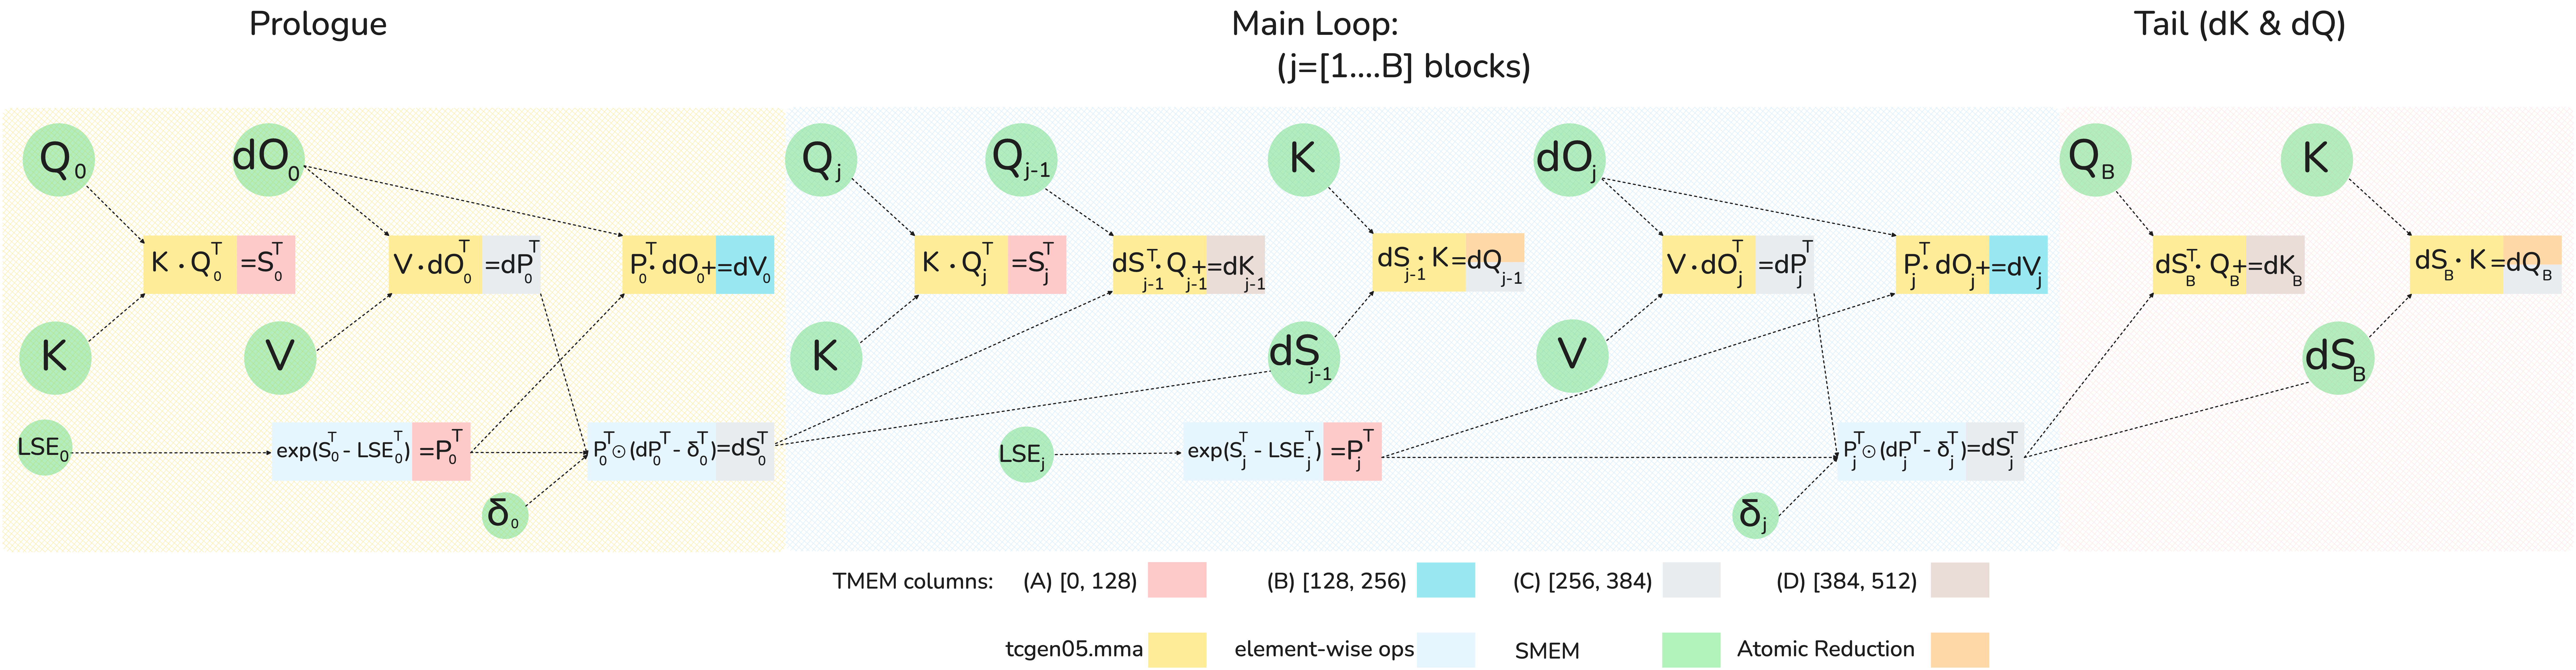
\includegraphics[width=1.0\linewidth]{Figures/fa_bwd_p8.png}
  \caption{FlashAttention-4 backward computation graph (5 MMA operations + 2 elementwise operations), showing the 1-CTA MMA mode software pipeline order across the prologue, main loop, and tail.}
  \label{fig:bwd_computational_graph}
\end{figure*}




\noindent\textbf{Exponential unit.}
The exponential unit computes elementwise operations (exponentials, logarithms, and related nonlinear functions) required for the softmax and its gradient. The backward pass requires exponential operations on the $M \times N$ values (corresponding to the attention matrix $\vS$ and related terms). With a throughput of 16 operations per cycle, the exponential unit requires
{\setlength{\abovedisplayskip}{1pt}%
 \setlength{\belowdisplayskip}{1pt}%
 \setlength{\abovedisplayshortskip}{1pt}%
 \setlength{\belowdisplayshortskip}{1pt}%
\begin{equation}
    T_{\text{exp}} = \frac{MN}{16} \text{ cycles}.
\end{equation}}
Table~\ref{tab:bwd_roofline} summarizes the analysis for the typical tile configuration $M = N = d = 128$. The shared memory traffic time of 3328 cycles exceeds both the MMA compute time (2560 cycles) and the exponential unit time (1024 cycles), indicating that shared memory bandwidth is the primary bottleneck, though less severely than global memory traffic would suggest. This motivates our kernel design to maximize overlap between MMA operations and other computations to hide shared memory latency.

\begin{table}[t]
\centering
%\resizebox{\columnwidth}{!}{
\begin{tabular}{lcc}
\toprule
Resource & Cycles ($N = d = 128$) & Cycles ($N = d = 128$) \\
         & \textbf{1-CTA} ($M = 128$) & \textbf{2-CTA} ($M = 256$) \\
\midrule
MMA compute & 2560 & 2560 \\
Shared memory (MMA operands) & 2048 & 1536 \\
Shared memory ($\vdS$ write) & 256  & 256 \\
Shared memory ($\vdS$ \textit{DSMEM}) & 0 & 384 \\
Shared memory ($\vdQ$ write + read) & 1024 & 512 \\
%\cmidrule(lr){2-2}
\textbf{Total shared memory} & \underline{\textbf{3328}} & \underline{\textbf{2688}} \\
Exponential unit & 1024 & 1024\\
\bottomrule
\end{tabular}
%}
\caption{Roofline analysis for the attention backward pass with $M = N = d = 128$. Shared memory traffic is the bottleneck, exceeding MMA compute time by approximately 30\%. In the 2-CTA setting with $M =256$ and $N = d = 128$ (with an exception to the $\vdQ$ mma, with $M = N =128$ and $d=256$), shared memory traffic exceeds MMA compute time by approximately 5\%.}
\label{tab:bwd_roofline}
%\vspace{-20pt}
\end{table}

\subsubsection{New pipeline to overlap matmul and softmax}

The backward pass in flash attention performs five MMA operations, corresponding to recomputing $\vS$, and the two gradient computations induced by $\vQ \vK$ (which yields $\vdQ$ and $\vdK$) and $\vP \vV$ (which yields $\vdP$ and $\vdV$) respectively.
In FA-3, accumulators are stored in registers and registers are a limited resource.
This imposes significant ordering constraints that---in effect---serialize the compute graph, i.e.,  compute $\vS, \vdP, \vdV, \vdQ, \vdK$, with only the TMA load running significantly out of turn.
In addition to that, the algorithm is similar:
It iterates along the KV sequence length dimension and computes values transposed w.r.t. the forward pass, since that is the layout that the $\vdV$ and $\vdK$ gradient calculations require to read one of their operands from tensor memory.
$\vdQ$ accumulates through the atomics.

In FA-4, TMEM enables additional schedules compared to FA-3 that provide significant overlap between MMA and non-MMA operations.
Specifically, just as with the forward pass, we are trying to hide the latency of the softmax calculation.
In FA-3, the softmax computation overlaps with the MMA for $\vdP$.
From the previous section, we know that on Blackwell we need at least two MMA operations to run concurrently.

We achieve this by using the $\vdQ$ and $\vdK$ MMA's of the previous iteration.
This requires careful management of shared memory and tensor memory resources between loading, MMA, compute, and reduction operations.
In particular, note that we do not have sufficient tensor memory to fit five accumulator tiles.
At most, four tiles of 128 by 128 elements can fit and $\vdV$ and $\vdK$ accumulate, and thus cannot share their space.
In our implementation, we have $\vS$ and $\vP$ share one of the tmem blocks (at offset 0) and we have $\vdP$, $\vdS$ and $\vdQ$ share the other one. We demonstrate the computational graph of the FA-4 bwd in Figure~\ref{fig:bwd_computational_graph}. 


\begin{figure*}[t]
  \centering 
  %\hspace*{-3cm}
  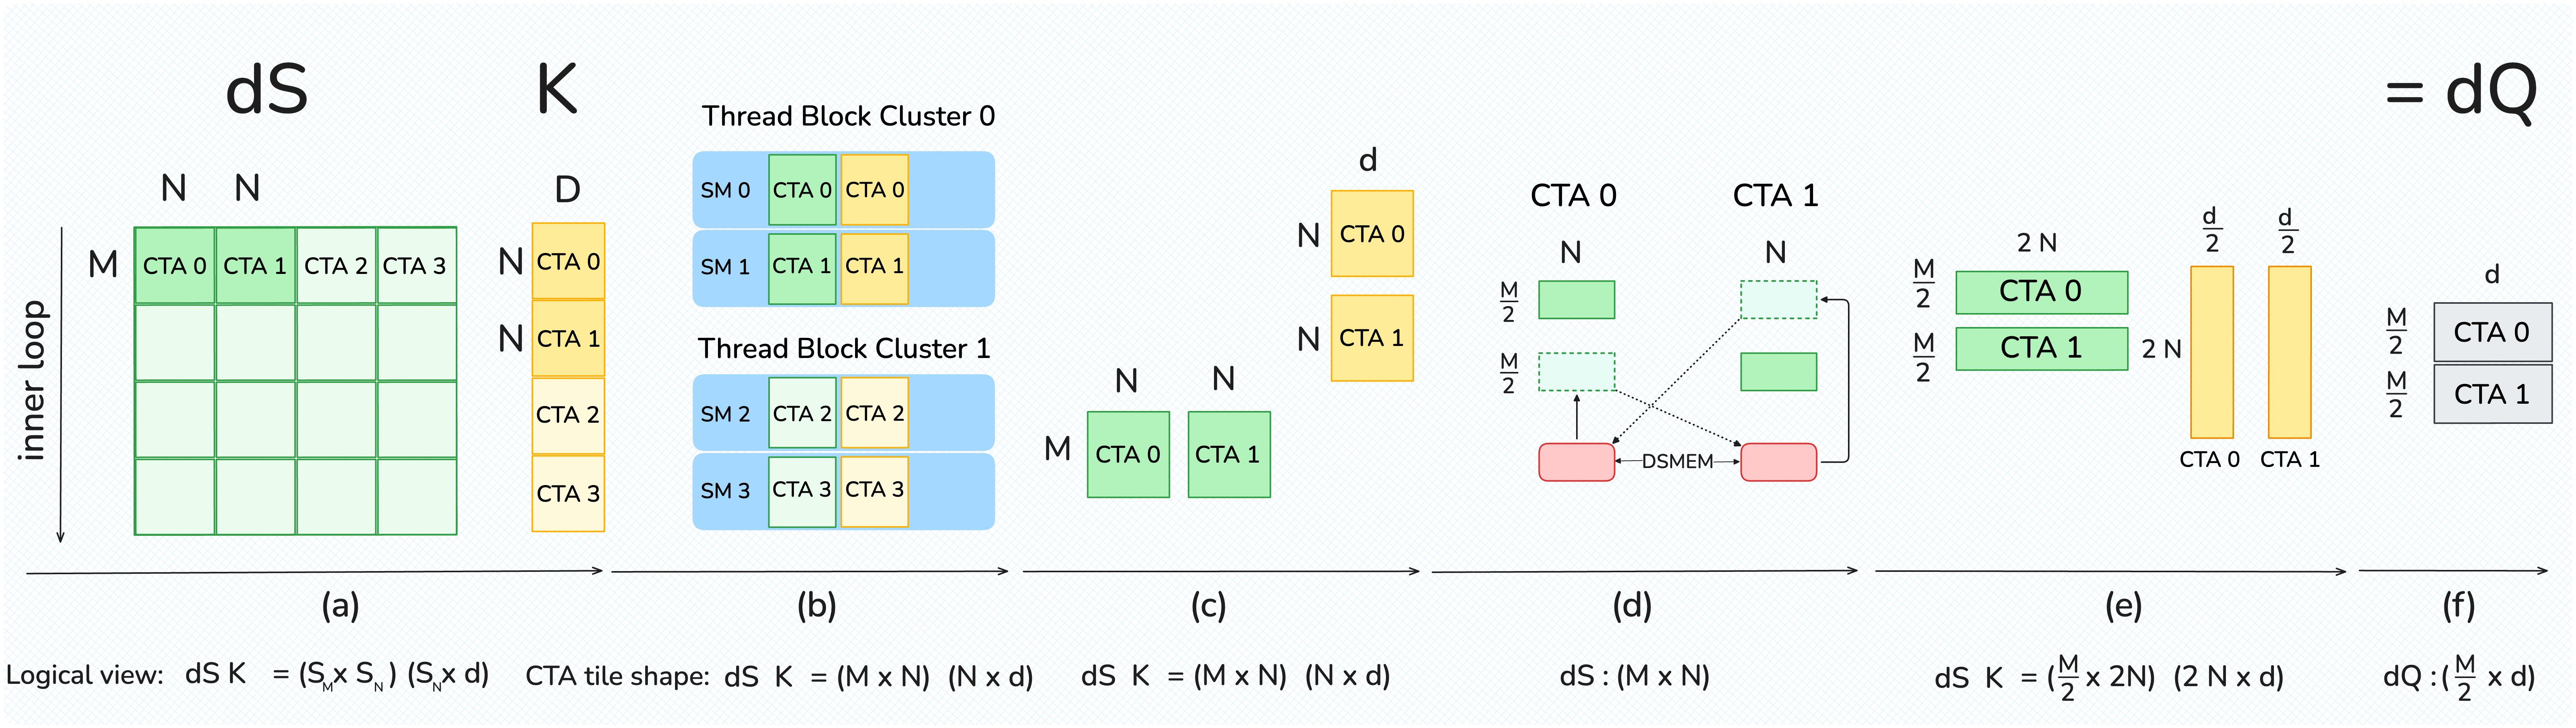
\includegraphics[width=1.0\linewidth]{Figures/2cta_figure.png}
  \caption{In the 2-CTA backward $dQ$ step, the CTA pair uses DSMEM to exchange half of the $dS$ tile so each CTA forms an $(\frac{M}{2} \times 2N)$ operand and can run a CTA-pair UMMA with a doubled reduction. 
}
  \label{fig:2cta_figure}
\end{figure*}


\subsubsection{2-CTA backward pass: Reducing shared memory traffic and global atomic adds}

Even with improved pipelining and with two of the ten GEMM operands resident in tensor memory, shared memory bandwidth still dominates the backward pass. Across the five GEMMs, the remaining eight BF16 operands are loaded from shared memory to feed the tensor cores, and this shared memory traffic incurs about 30\% more cycles than the tensor core compute. To further mitigate this bottleneck, we use the 2-CTA MMA mode introduced by Blackwell, in which the output accumulator is partitioned in the M dimension. With an MMA tile shape of $M=256$ and $N=K=128$, the two CTAs act as a single larger tile: each CTA loads and stages half of operand B and keeps only its own accumulator slice.

\textbf{Shared memory traffic}. With five GEMMs in the backward pass, we use MMA tile shape of $M=256$ and $N=K=128$, which roughly halves the shared memory traffic for operand B. In the FlashAttention backward pass, each CTA holds a fixed KV tile (parallelize the outer loop across $N$ CTAs) and streams over M tiles in the inner loop. The accumulation of $\vdQ$ is a reduction in the KV sequence in the outer loop, but the 2-CTA MMA only splits the output tile, not the reduction axis, and the reduction dimension of the $\vdQ$ MMA is $N$, which is naturally split across the CTA pair. As a result, each CTA still needs the full reduction for the rows it owns. To address this conflict on the reduction axis, we use distributed shared memory (DSMEM) to exchange half of the dS between the two CTAs since they are in the same cluster.  This approach repacks $\vdS$ so that it is partitioned along the non-reduction axis, with each CTA owning its $\frac{M}{2}$ rows and holding the full $2N$ reduction. As a result, the per CTA $\vdQ$ MMA tile shape is ($\frac{M}{2}, 2N)(2N, d)$ and accumulates a tile ($\frac{M}{2}, d$) in tensor memory. In 2-CTA MMA mode, the MMAs for $\vS$, $\vdP$, $\vdV$ and $\vdK$ run with the tile $M=256$, while $\vdQ$ uses $M=128$ but with double reduction $2N=256$.  We then reordered the software pipeline with respect to the 1-CTA variant to hide the DSMEM latency. We compute $\vdP$ for the current tile before computing $\vdQ$ for the tile of the previous iteration. The $\vdQ$ tile is small enough to fit in TMEM alongside $\vP$, reusing the same TMEM region as $\vS$, so we no longer reuse the same TMEM region for $\vdP$ and $\vdQ$ as we do in the 1-CTA mode. With this new pipelining ordering, we can compute the element-wise $\vdS$ of the current tile in parallel with the $\vdQ$ MMA of the tile from the previous iteration. See Figure~\ref{fig:2cta_figure} for an illustration of how the $\vdQ$ step is decomposed.

\textbf{$\vdQ$ atomic adds}. A complementary benefit of this $\vdQ$ decomposition is that it halves the number of global atomic reductions. Atomic updates introduce nondeterminism and are expensive as they occur in every iteration of the inner loop. Consequently, each CTA writes only half of the $\vdQ$ tile and performs half as many global atomic reductions as the 1-CTA counterpart.



\subsubsection{Deterministic backward pass} 

Our backward kernel introduces nondeterminism for the gradient computation due to inter-CTA reductions in global memory (affecting $\vdQ$ in general, and $\vdK$/$\vdV$ in the case of GQA). To ensure reproducibility and facilitate reliable debugging during training, we also provide a deterministic execution mode. The standard solution, which we also adopt, is to serialize the global reductions using a semaphore lock. Specifically, each CTA writing to a common $\vdQ$ tile must acquire the lock according to a predefined order, perform its reduction, and then release the lock by incrementing the semaphore counter. 

This lock-based approach impacts performance for two main reasons: (1) issuing the memory fence to ensure device-wide visibility of the semaphore write (required for correct acquire--release semantics), and (2) introducing stalls as each CTA waits for previous CTAs reducing on a common $\vdQ$ tile to complete. In load-imbalanced situations, a naive choice of CTA order can severely degrade performance. In general, we do CTA swizzling in the head and batch dimensions to reduce stalls (up to L2 cache capacity, cf. \cref{sec:algo_other}). For causal masking, we additionally launch KV blocks in descending order, traverse query blocks in ascending order starting from the diagonal, and order the $
\vdQ$ reductions by descending query block index. This ``shortest-processing-time-first'' (SPT) schedule ensures that no CTA is stalled on its first $\vdQ$ write.

